\subsection*{Question 3.4}
The plot of the SVD.samples, can be seen in figure \ref{fig:q34}. It can be seen of the graf, that some of the gene group together, like the MEL gene type, at the top of the figure. The gene type BRE can be seen grouping together whit all of the otter gene type, and is not confined to are small group, like the other This indicate that this gene type can be are miss classification or that it just the way this gene type blend.
\begin{figure}[!htbp]
  \centering
  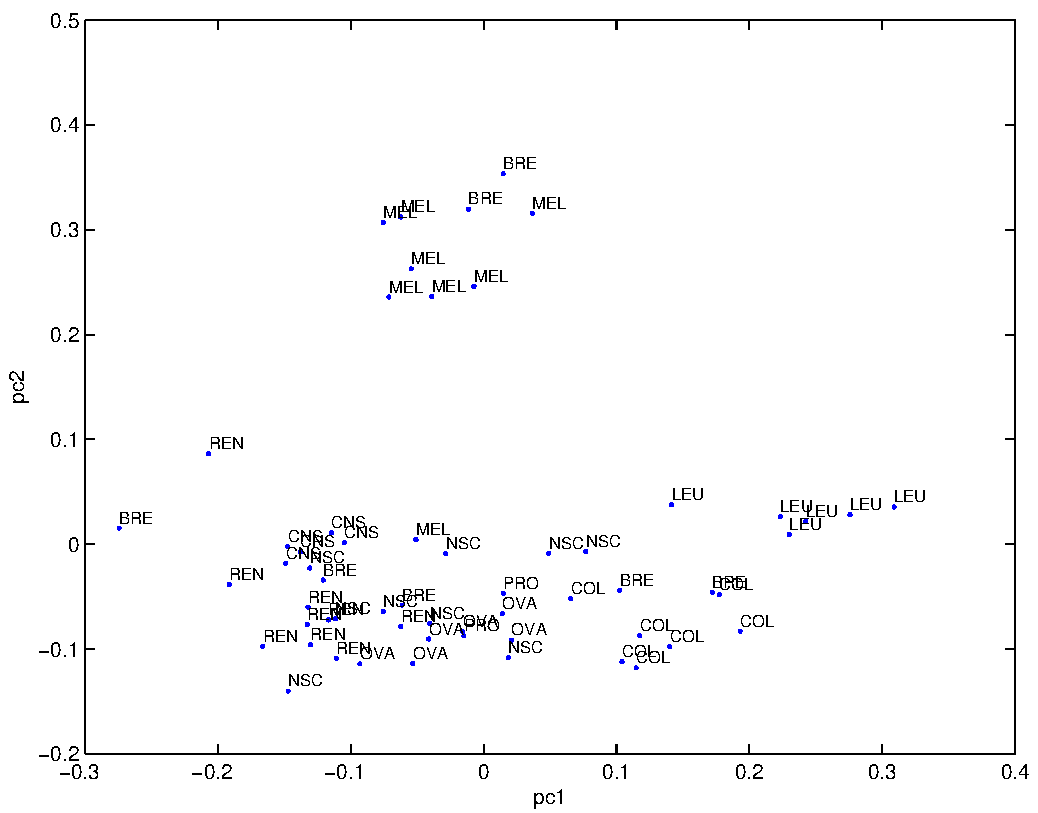
\includegraphics[width=0.85\textwidth]{./images/q34cancer}
  \caption{Shows are plot over the SVD sample of difference gene.}
  \label{fig:q34}
\end{figure}

